% Created 2014-09-18 Thu 14:04
\documentclass[11pt]{article}
\usepackage[utf8]{inputenc}
\usepackage[T1]{fontenc}
\usepackage{graphicx}
\usepackage{longtable}
\usepackage{float}
\usepackage{wrapfig}
\usepackage{soul}
\usepackage{amssymb}
\usepackage{hyperref}


\title{Web Performance Fundmentals}
\author{jatin}
\date{18 September 2014}

\begin{document}

\maketitle

\setcounter{tocdepth}{3}
\tableofcontents
\vspace*{1cm}
\section{Objective}
\label{sec-1}

\begin{itemize}
\item Understanding working of a webpage
\item Critical Rendering Path
\item Analysis and Optimization
\item Hands-on with chrome dev tools
\item Hands-on wit pagespeed, yslow and webpagetest
\end{itemize}
\section{Working of Webpage}
\label{sec-2}

\subsection{From Hypertext document to complex Web Application}
\label{sec-2.1}

\begin{itemize}
\item Plain hypertext document with text and hyperlink to other hypertext documents
\item Web page with images, audio and styling of tags.
\item Web application <==> Webpage + JavaScript
\end{itemize}
\subsection{Dependency Graph}
\label{sec-2.2}

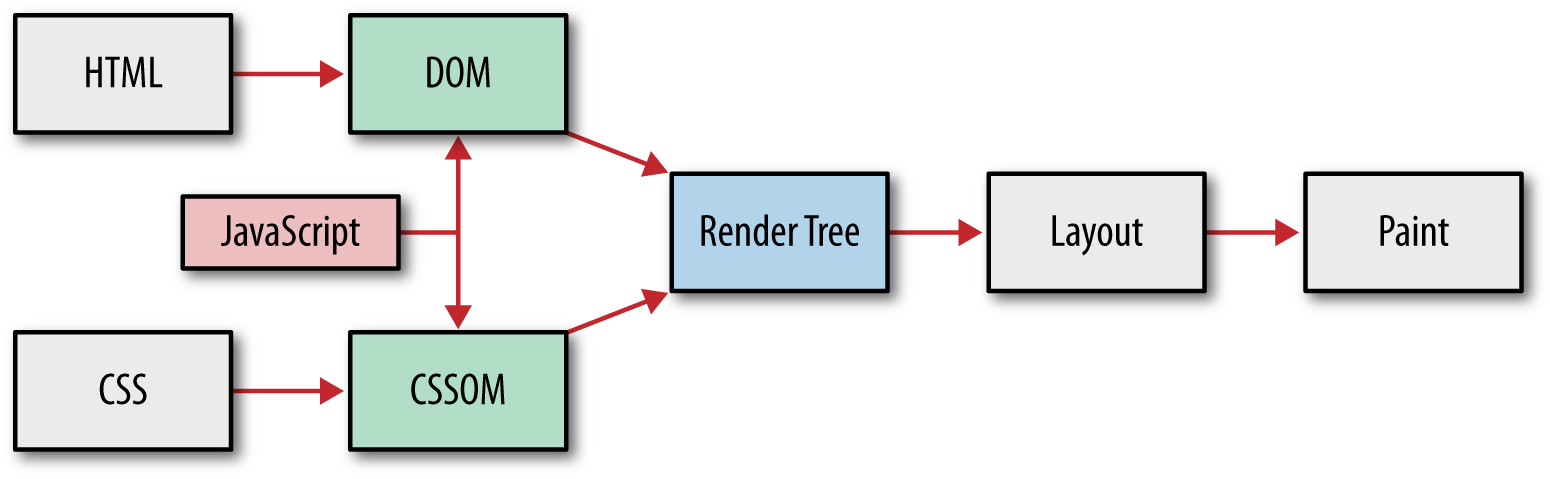
\includegraphics[width=10em]{/home/jatin/Documents/yslow-framework/documentation/dependency-graph.png}
\subsection{Critical Rendering Path}
\label{sec-2.3}

\begin{figure}[ht]
 \centering
  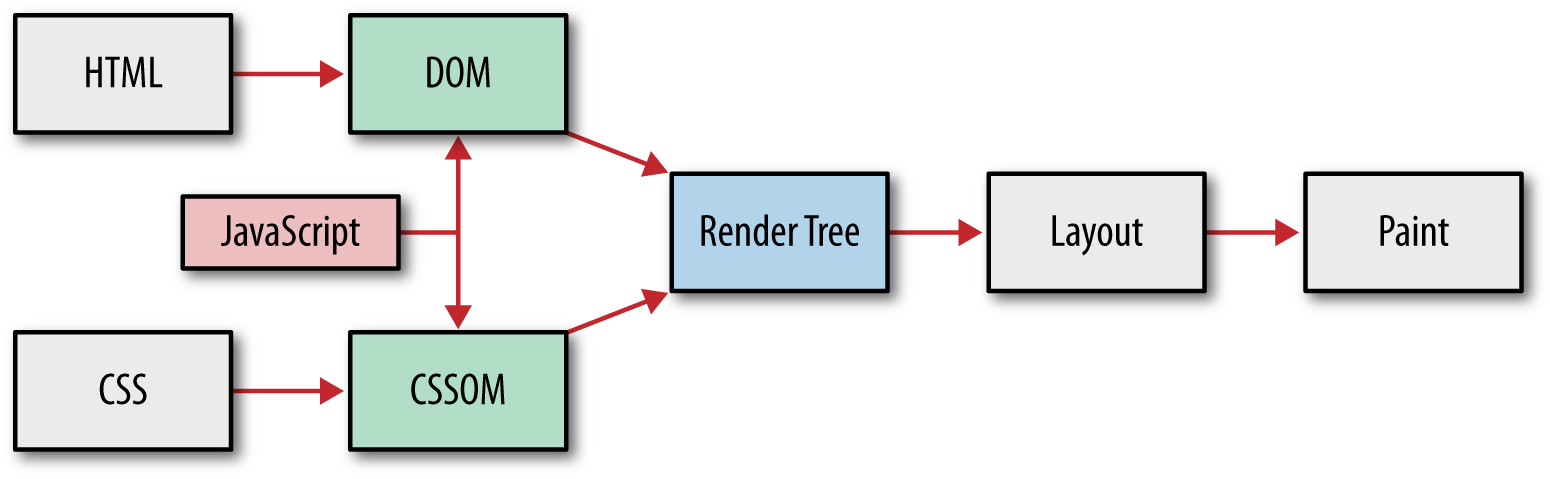
\includegraphics[scale=0.5]{/home/jatin/Documents/yslow-framework/documentation/dependency-graph.png}
\caption{Number of urls versus Use a Content Delivery Network (CDN)}    
\label{fig:dg}
\end{figure}   

\end{document}
